\documentclass[12pt,]{article}
\usepackage[utf8]{inputenc}
\usepackage[T1]{fontenc}
\usepackage{mathptmx}
\usepackage{geometry}
\usepackage{mathtools}
\usepackage[english]{babel}
\usepackage{graphicx}
\usepackage{stackengine}
\usepackage[os=win]{menukeys}
\usepackage{hyperref}
\usepackage{minted}
\usepackage{xcolor}
\usepackage{tikz}
\usepackage[yyyymmdd,hhmmss]{datetime}

\newcommand{\ShowOsVersion}{
	\immediate\write18{\unexpanded{foo=`uname -sro` && echo "${foo}" > tmp.tex}}
			\input{tmp}\immediate\write18{rm tmp.tex}
			}
			
\newcommand{\ShowTexVersion}{
			\immediate\write18{\unexpanded{foo=`pdflatex -version | head -n1 | cut -d' ' -f1,2` && echo "${foo}" > tmp.tex}}
	\input{tmp}\immediate\write18{rm tmp.tex}
}

\addto\captionsenglish{\renewcommand{\contentsname}{Daftar Isi}}

\hypersetup{
	colorlinks=true, %set true if you want colored links
	linktoc=all,     %set to all if you want both sections and subsections linked
	linkcolor=blue,  %choose some color if you want links to stand out
}

\geometry{
	legalpaper,
	left=15mm,
	right=10mm,
	top=10mm,
	bottom=15mm,
}

\title{\Large \bf
	Preliminary Design Report\\
	\small{(Evaluation Purpose)}
}

\author{Achmadi ST MT}

\date{}

\definecolor{LightGray}{gray}{0.9}

\begin{document}
	\maketitle
	\thispagestyle{empty}
	
	\vspace{125pt}
	\begin{figure}[!ht]
		\centering
		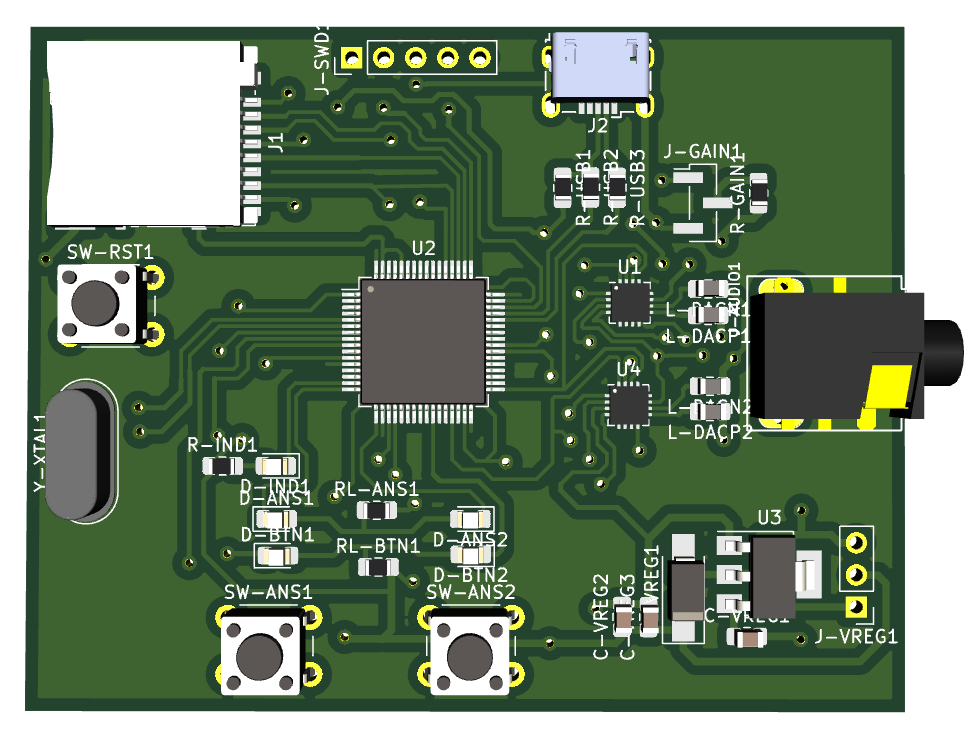
\includegraphics[width=500pt]{images/end_stm32f401re}
	\end{figure}
	
	\vspace*{175pt}
	\noindent This report written using: \\
	OS : \ShowOsVersion \\
	TeX : \ShowTexVersion \\
	Update: {\today} at \currenttime \\
	
%%%%%%%%%%%%%%%%%%%%%%%%%%%%%%%%%%%%%%%%%%%%%%%%%%%%%%%%%%%%%%%%%	
	
	\newpage
	\tableofcontents
	
%%%%%%%%%%%%%%%%%%%%%%%%%%%%%%%%%%%%%%%%%%%%%%%%%%%%%%%%%%%%%%%%%
	
	\newpage
	\section{Preliminary Design}
	
	Berikut akan dijelaskan desain circuit untuk beberapa versi,
	yaitu versi \textbf{Developmen}t, versi \textbf{Low-Fab}, dan versi \textbf{High-Fab}.  
	
	\subsection{Design Requirements}
	
	Beberapa alasan/kebutuhan pembagian versi desain ini antara lain:
	
	\subsubsection{PCB Fabrication}
	
	Beberapa alasan terkait untuk PCB Desain antara lain:
	\begin{itemize}
		\item \textbf{Vias.}\\
		Vias adalah bagian PCB untuk penyambung/jembatan antara jalur atas dan jalur bawah.
		Ukuran vias bervariasi antara 0.8mm hingga 1.6mm dengan ukuran lubang 0.4mm hingga 0.8mm.
		Vias dapat diisi dengan timah+wire dengan solder secara manual, maupun tembaga saat proses fabrikasi.
		Semakin banyak jumlah vias, maka assembly komponen ke PCB akan memakan waktu lama jika dikerjakan manual.
		
		\begin{figure}[!ht]
			\centering
			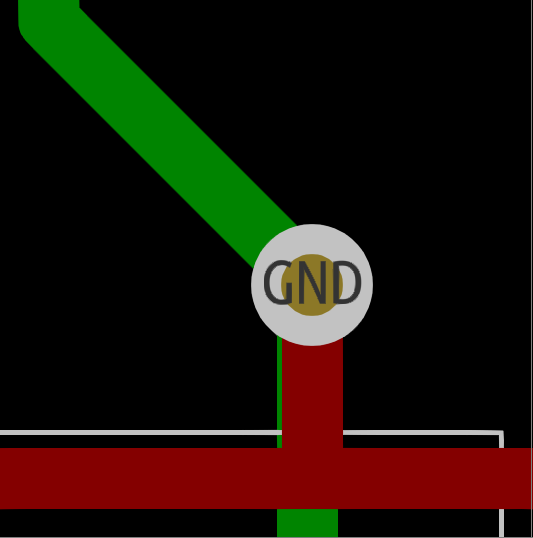
\includegraphics[width=125pt]{images/vias_layout}
			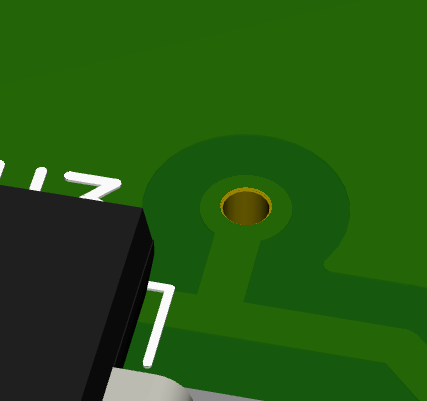
\includegraphics[width=125pt]{images/vias_pcb}
			\caption{Contoh Vias dalam (kiri) layout dan (kanan) PCB}
		\end{figure}
	
		\item \textbf{Minimum Clearance.}\\
		Minimum Clearance adalah jarak terkecil antara 2 jalur (wire/line) yang berbeda sinyal/power.
		Tidak hanya jalur, melainkan juga pads pada komponen.
		PCB House/Manufaktur lokal Indonesia pada umumnya mampu hingga clearance 0.5mm.
		
		\begin{figure}[!ht]
			\centering
			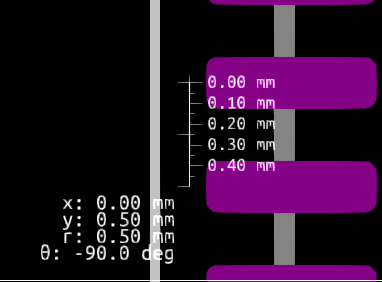
\includegraphics[width=125pt]{images/pcb_minMAX98}
			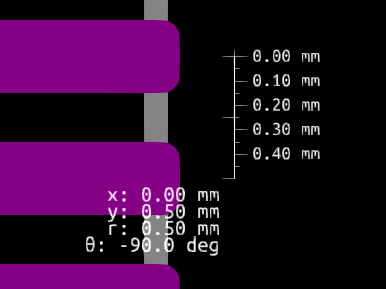
\includegraphics[width=125pt]{images/pcb_minSTM32}
			\caption{Contoh minimum clearance pin untuk chip (kiri) MAX98357A dan (kanan) STM32}
		\end{figure}
	
		\item Masking.
		Masking adalah lapisan tipis permanen untuk menutupi permukaan PCB dan jalur/line/wire tembaga.
		Masking hanya menyisakan bagian tembaga yang pads komponen untuk soldering.
		Komponen dengan paket-paket SMD yang memerlukan teknik solder hot-air wajib menggunakan PCB ber-masking.
		
		\begin{figure}[!ht]
			\centering
			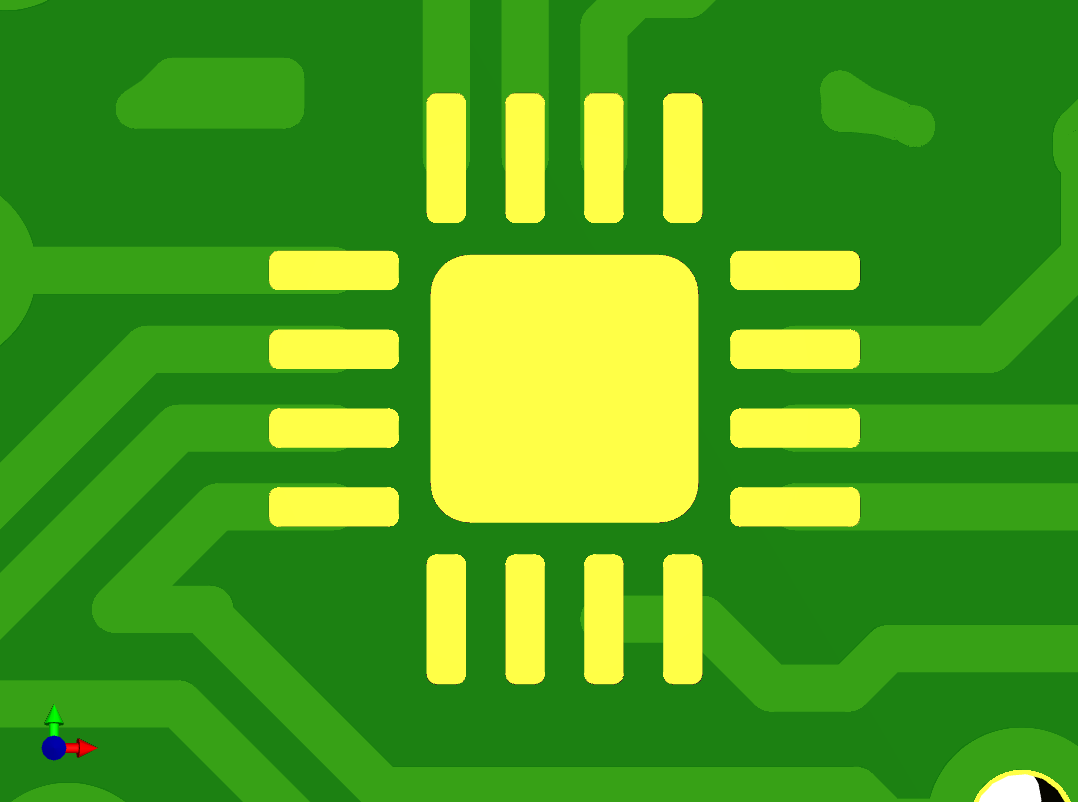
\includegraphics[width=125pt]{images/pcb_masked}
			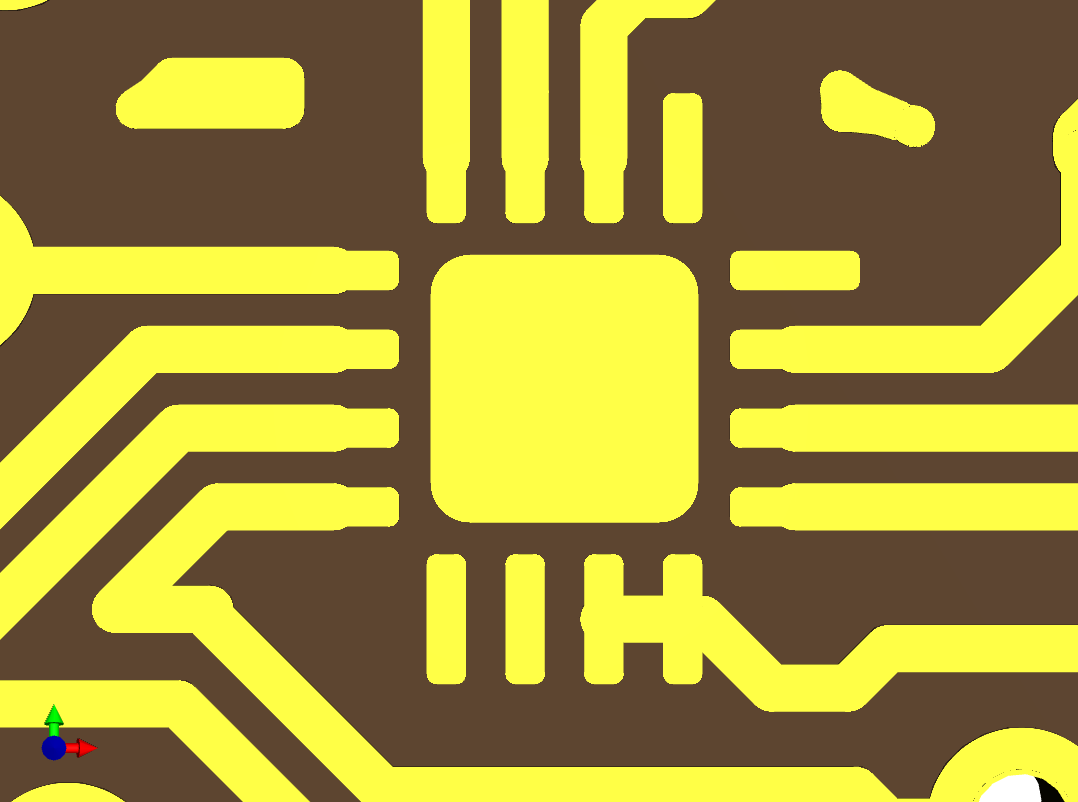
\includegraphics[width=125pt]{images/pcb_unmasked}
			\caption{Contoh PCB dengan (kiri) masked dan (kanan) unmasked}
		\end{figure}
		
	\end{itemize}

	\newpage
	\subsubsection{Component Packages}
	
	Component packages adalah jenis paket komponen yang dipakai dan kaitannya terhadap kebutuhan teknik soldering.
	Untuk menghemat space, maka seluruh komponen pasif (Resistor, Capasitor, Inductor) menggunakan paket SMD 0805 dengan ukuran 2mm x 1.5mm. 
	Walaupun cukup kecil, namun masih dapat disolder manual menggunakan solder biasa dan timah pasta. 
	
	Begitu juga dengan chip STM32F yang menggunakan paket QFP-64 dengan pin-clearance 0.5mm,
	masih dapat disolder manual dengan solder biasa dan timah pasta. 
	
	\begin{figure}[!ht]
		\centering
		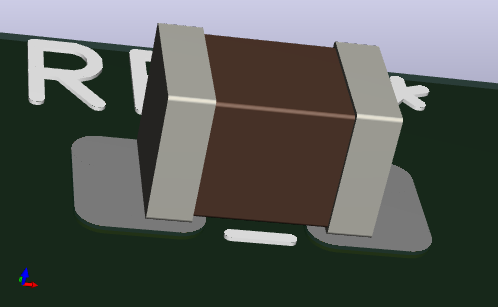
\includegraphics[width=125pt]{images/smd_0805}
		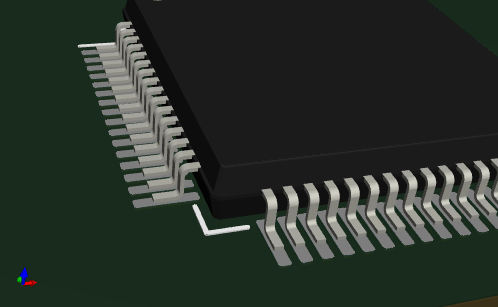
\includegraphics[width=125pt]{images/smd_qfp64}
		\caption{Contoh paket yang masih dapat disolder manual dengan solder biasa, yaitu (kiri) 0805 dan (kanan) QFP-64}
	\end{figure}

	Berbeda jika komponen menggunakan paket dengan pin yang tidak ter-\textit{expose} dari fisik chip,
	atau panjang pin sangat pendek (tidak sampai 1mm).
	Sebagai contoh chip MAX98357A yang menggunakan paket QFN-16 dengan ukuran 2x2 mm.
	Maka untuk komponen seperti ini diperlukan teknik soldering hot-air dan timah pasta.
	Disini masih bisa dipaksakan menggunakan solder biasa dan timah pasta, namun hasilnya diragukan kualitasnya.
	
	\begin{figure}[!ht]
		\centering
		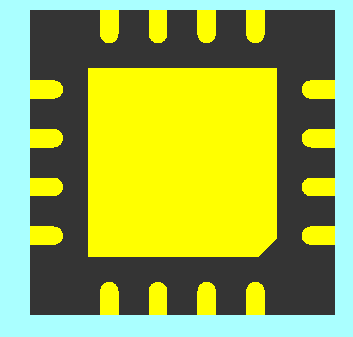
\includegraphics[width=200pt]{images/qfn16-bottom}
		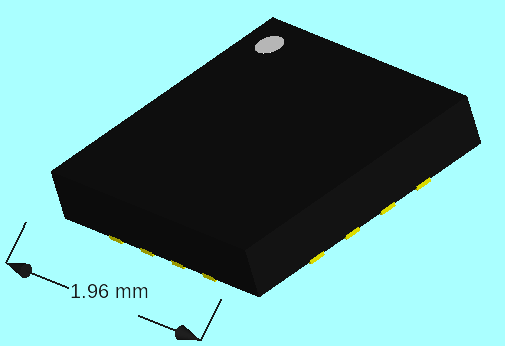
\includegraphics[width=200pt]{images/qfn16-ortho}
		\caption{Contoh paket yang direkomendasikan menggunakan teknik solder hot-air, yaitu QFN-16}
	\end{figure}

	Untuk solder hot-air, dibutuhkan set solder stttion dengan harga yang seringkali jauh lebih mahal dibandingkan solder iron biasa.
	 
	\begin{figure}[!ht]
		\centering
		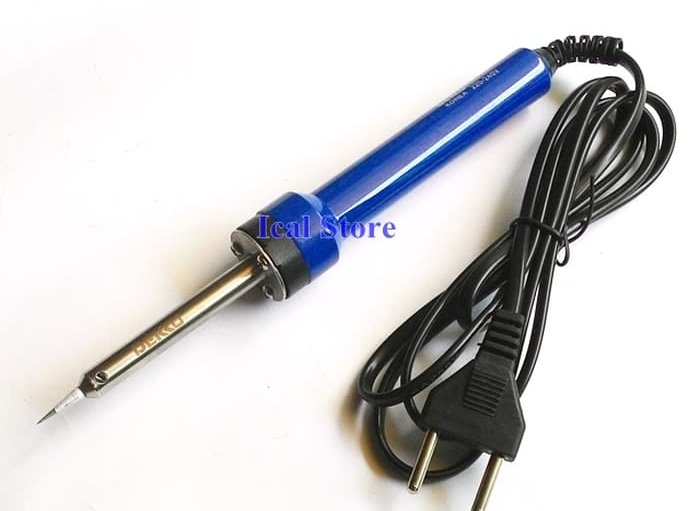
\includegraphics[width=200pt]{images/solder_iron}
		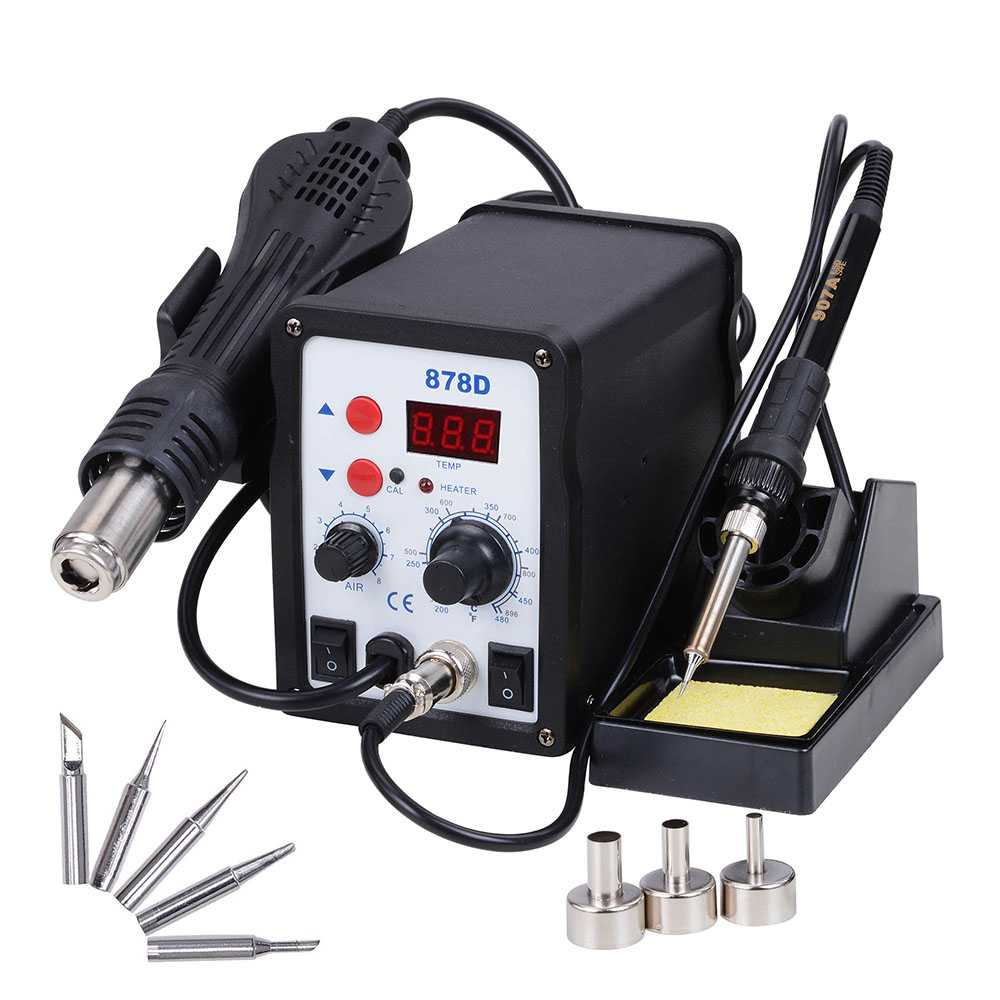
\includegraphics[width=200pt]{images/solder_station}
		\caption{Contoh (kiri) Solder Iron dan (kanan) Solder Station yang dilengkapi Solder Hot-Air}
	\end{figure}
	
%%%%%%%%%%%%%%%%%%%%%%%%%%%%%%%%%%%%%%%%%%%%%%%%%%%%%%%%%%%%%%%%%

	\newpage
	\subsection{Development Version}
	
	Versi Development ini adalah versi yang menggunakan board STM32 Nucleo sebagai dasar.
	Versi ini berformat PCB Shield untuk board Nucleo.
	
	\subsubsection{Features}
	\begin{figure}[!ht]
		\centering
		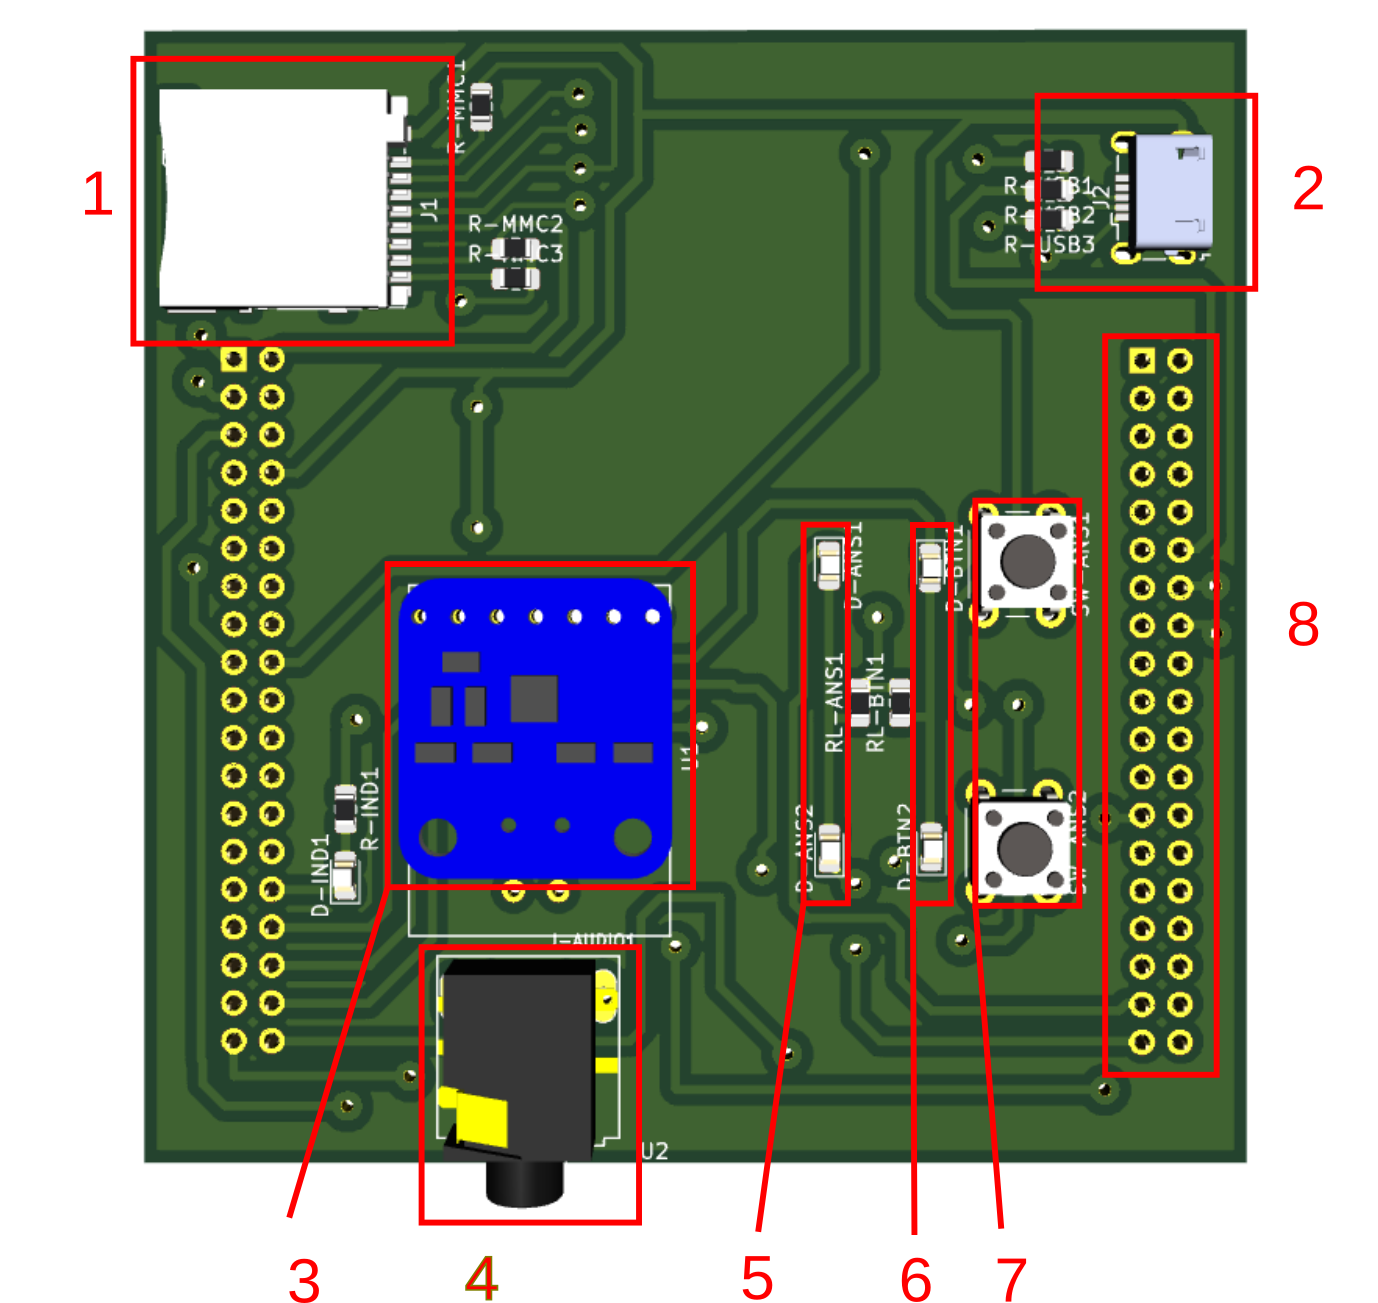
\includegraphics[width=500pt]{images/vdev.png}
		\caption{Fitur dalam desain}
	\end{figure}

	Berikut adalah daftar fitur yang telah tersedia dalam desain:
	\begin{enumerate}
		\item \textbf{MicroSD slot.}\\
		Digunakan untuk menyimpan rekaman setiap sesi test dalam bentuk file teks.
		Format data dapat berupa CVS, XML, JSON, atau format data yang dibuat sendiri sesuai kebutuhan.
		
		\item \textbf{USB-Port.}\\
		USB Port untuk komunikasi dengan standar USB-CDC (Communication Device Class), yaitu emulasi komunikasi data serial.
		Kompatibel dengan driver ACM (Abstract Control Model) untuk Unix (Android/Linux) dan Usbser.sys untuk Windows.\\
		Beberapa varian board Nucleo-64 juga menyediakan USB-OTG-FS Host untuk handle USB Flash-Disk (implementasinya sedang direncanakan).
		
		\newpage
		\item \textbf{Max98357A Board.}\\
		Audio DAC (Digital to Analog Converter) MAX98357A adalah \textbf{Mono Class-D} amplifier untuk menghasilkan Audio output dengan input
		PCM (Pulse-Coded Modulation) standar I2S (Inter-IC Sound).\\
		\textbf{Spesifikasi}: 86-11800 Hz dan 98-42 dB pada default amplifikasi 9dB (Diukur menggunakan KEMAR-set dan Audio-Box BSWA).
		
		\item \textbf{Jack Audio.}\\ 
		Jack Audio 3.5mm dengan konfigurasi pin TRS (Tip,Round,Sleeve) dan kompatibel untuk jack TRRS OMTP/Nokia.
		
		\item \textbf{LED True/False Indicator.}\\
		LED ukuran SMD 0805 sebagai indikator jawaban salah atau benar.
		
		\item \textbf{LED Answer Options Indicator.}\\
		LED ukuran SMD 0805 sebagai indikator jawaban pilihan jawaban untuk user.
		
		\item \textbf{User-Button Answer Options.}\\
		Tombol untuk input user terhadap jawaban.
		
		\item \textbf{Nucleo Pin-Header.}\\
		Konektor untuk penyambung antara PCB Shield dengan board STM32 Nucleo.
	\end{enumerate}

	\subsubsection{Power-Compats}
	Untuk power, PCB Shield ini tidak menggunakan power secara menyendiri, melainkan mengambil power dari board STM32 Nucleo.
	Sedangkan untuk STM32 Nucleo sendiri menggunakan power 5V dari USB ter-regulasi.
	
	Board STM32 Nucleo yang kompatibel adalah varian Nucleo-64 meliputi:
	\begin{itemize}
		\item Nucleo-F072RB.
		\item Nucleo-F091RC. 
		\item Nucleo-F303RE.
		\item Nucleo-F401RE (Recommended).
		\item Nucleo-F411RB.
		\item Nucleo-F446RE.
	\end{itemize}

	\begin{figure}[!ht]
		\centering
		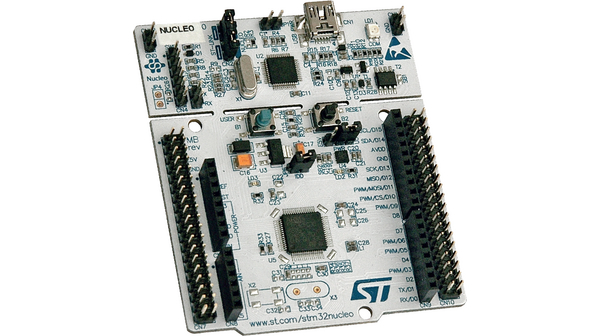
\includegraphics[width=255pt]{images/nucleof401}
		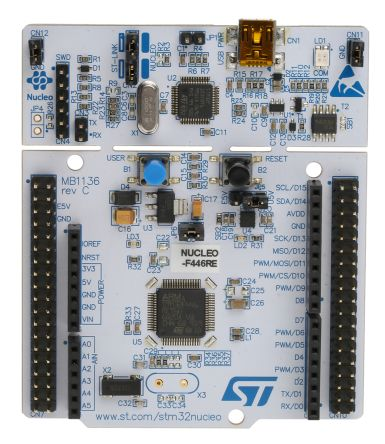
\includegraphics[width=150pt]{images/nucleof446}
		\caption{Contoh Board Nucleo64 dengan chip (kiri) STM32F401RE dan (kanan) STM32F446RE}
	\end{figure}

	\newpage
	\subsubsection{Pro-Con}
	Berikut adalah beberapa poin keuntungan dan kerugian dari versi ini:\\
	
	\textbf{Pros}:
	\begin{itemize}
		\item Board Nucleo64 sebagai main-board memiliki standar yang konsisten di semua varian dan ketersediaan lokal yang tinggi.
		
		\item PCB shield sebagai wadah modul, tidak membutuhkan proses fabrikasi PCB yang tinggi dan tidak perlu masking.
		Percetakan/Etching PCB lokal Surabaya secara umum mampu fabrikasi dan cenderung murah.
		
		\item PCB shield cenderung mudah untuk dimodifikasi ulang.
		Cocok untuk tujuan evaluasi seperti prototyping/development maupun tugas-akhir.
	\end{itemize}

	\textbf{Cons}:
	\begin{itemize}
		\item Membutuhkan board lain (Nucleo64 board).
		\item Pertimbangan size dan space, hanya pas untuk satu modul MAX98357A, sehingga hanya mampu mono audio.
		\item Tidak \textit{user convenience}. 
	\end{itemize}

	\subsubsection{3D Mock-Up}
	\begin{figure}[!ht]
		\centering
		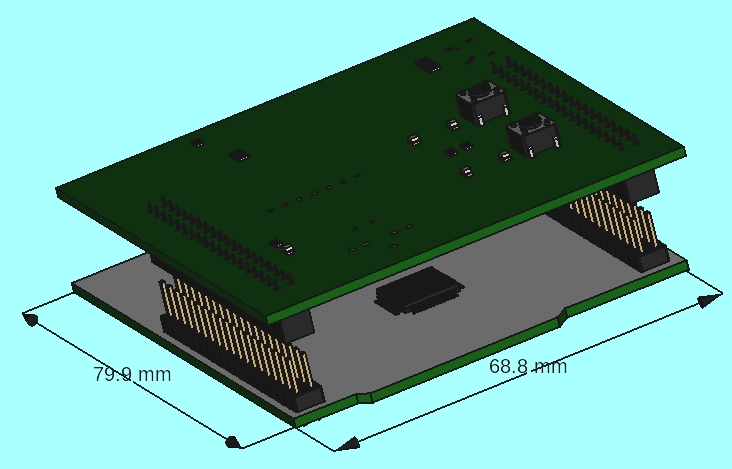
\includegraphics[width=400pt]{images/test1}
		\caption{Mock-Up 3D}
	\end{figure}

%%%%%%%%%%%%%%%%%%%%%%%%%%%%%%%%%%%%%%%%%%%%%%%%%%%%%%%%%%%%%%%%%

	\newpage
	\subsection{Low Fabrication Version}
	
	Versi Low-Fabrication ini adalah versi yang tidak perlu menggunakan board STM32 Nucleo sebagai dasar.
	Versi ini berformat standalone PCB dengan power regulator.
	
	\subsubsection{Features}
	\begin{figure}[!ht]
		\centering
		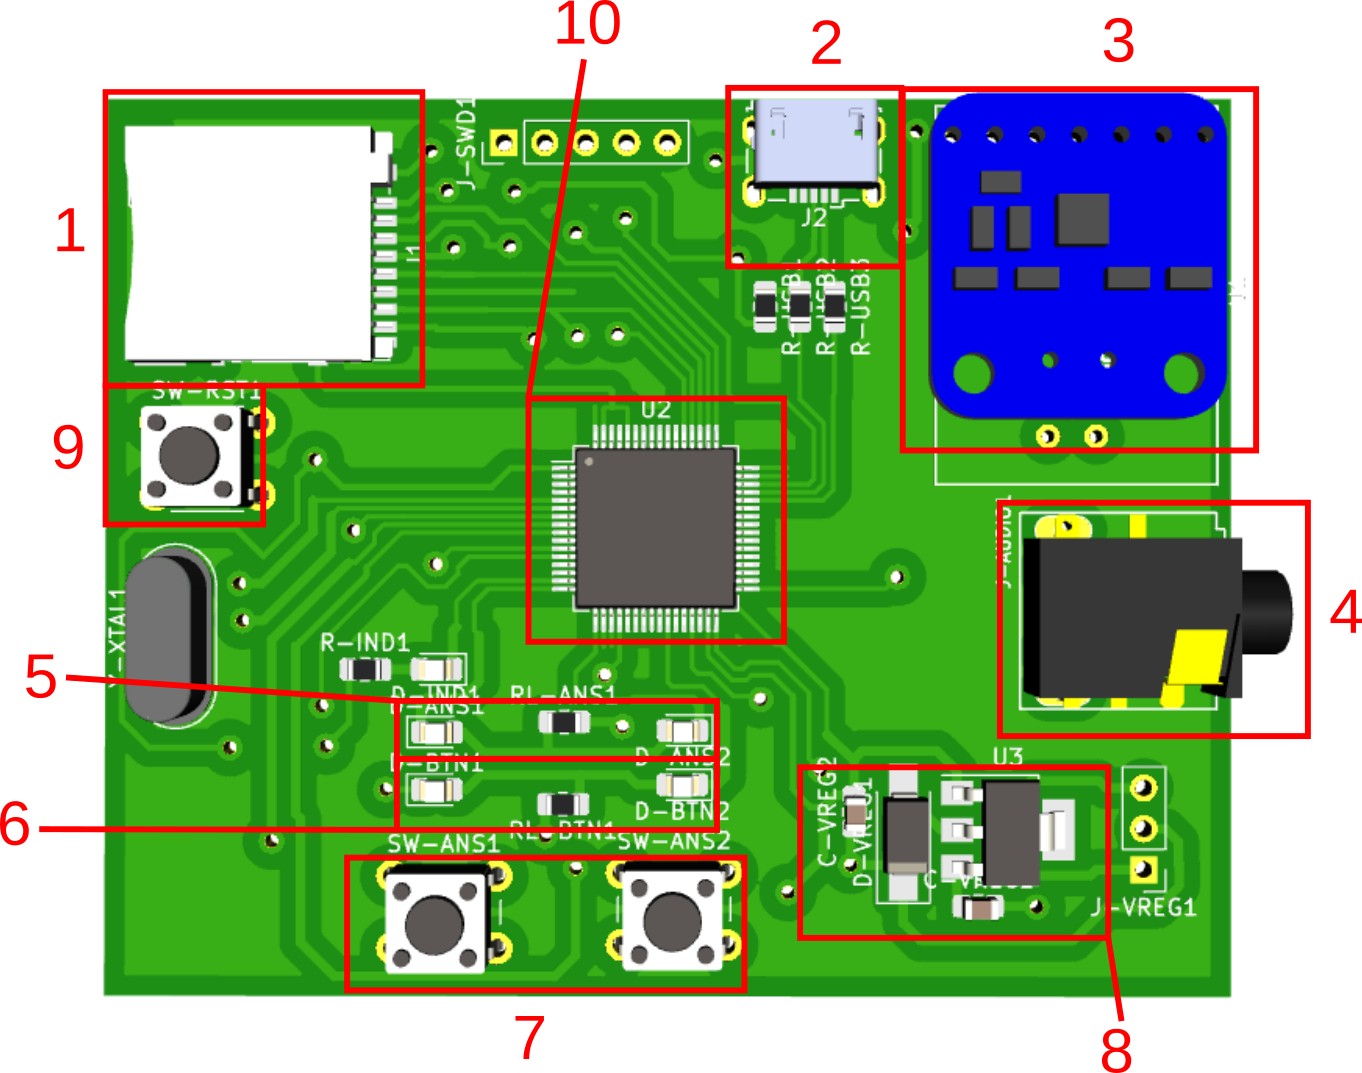
\includegraphics[width=500pt]{images/vlofab.png}
		\caption{Fitur dalam desain}
	\end{figure}

	Berikut adalah daftar fitur yang telah tersedia dalam desain:
	\begin{enumerate}
		\item \textbf{MicroSD slot.}\\
		Digunakan untuk menyimpan rekaman setiap sesi test dalam bentuk file teks.
		Format data dapat berupa CVS, XML, JSON, atau format data yang dibuat sendiri sesuai kebutuhan.
		
		\item \textbf{USB-Port.}\\
		USB Port untuk komunikasi dengan standar USB-CDC (Communication Device Class), yaitu emulasi komunikasi data serial.
		Kompatibel dengan driver ACM (Abstract Control Model) untuk Unix (Android/Linux) dan Usbser.sys untuk Windows.\\
		Beberapa varian main CPU chip juga menyediakan USB-OTG-FS Host untuk handle USB Flash-Disk (implementasinya sedang direncanakan).
		
		\newpage
		\item \textbf{Max98357A Board.}\\
		Audio DAC (Digital to Analog Converter) MAX98357A adalah \textbf{Mono Class-D} amplifier untuk menghasilkan Audio output dengan input
		PCM (Pulse-Coded Modulation) standar I2S (Inter-IC Sound).\\
		\textbf{Spesifikasi}: 86-11800 Hz dan 98-42 dB pada default amplifikasi 9dB (Diukur menggunakan KEMAR-set dan Audio-Box BSWA).
		
		\item \textbf{Jack Audio.}\\ 
		Jack Audio 3.5mm dengan konfigurasi pin TRS (Tip,Round,Sleeve) dan kompatibel untuk jack TRRS OMTP/Nokia.
		
		\item \textbf{LED True/False Indicator.}\\
		LED ukuran SMD 0805 sebagai indikator jawaban salah atau benar.
		
		\item \textbf{LED Answer Options Indicator.}\\
		LED ukuran SMD 0805 sebagai indikator jawaban pilihan jawaban untuk user.
		
		\item \textbf{User-Button Answer Options.}\\
		Tombol untuk input user terhadap jawaban.
		
		\item \textbf{Power/Voltage Regulator}\\
		Set voltage regulator berbasis IC AM1117 untuk regulasi tegangan input dari 5-12 volt ke VDD (3.3 volt) pada maksimal arus 1A.
		Battery monitor/charging circuit direncanakan masih menggunakan modul terpisah.
		
		\item \textbf{Reset Button.}\\
		Tombol input user untuk mengulang proses running/testing dari unit.
		
		\item \textbf{Main CPU STM32F-series.}\\
		Main microcontroller chip sebagai CPU. Menggunakan chip seri STM32F pada arsitektur ARM32 Cortex-M0/M3/M4.
		
	\end{enumerate}
	
	\subsubsection{Power-Compats}
	
	Untuk power, disediakan power regulator untuk regulasi dan konversi tegangan battery 3.7 hingga 12 volt ke 3.3 volt. 
	Pilihan untuk \textit{one-use} battery semisal battery PP3 (9v) atau AAA dalam 3-in-series,
	sedangkan untuk \textit{rechargable} battery dapat menggunakan 1000mAh dengan dilengkapi modul monitor/charging berbasis IC TP-4056.
	
	\begin{figure}[!ht]
		\centering
		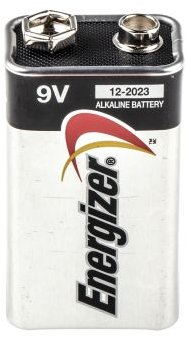
\includegraphics[width=50pt]{images/batt_pp3}
		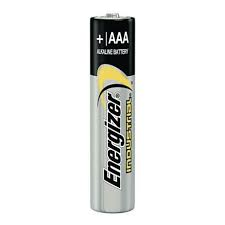
\includegraphics[width=100pt]{images/batt_aaa}
		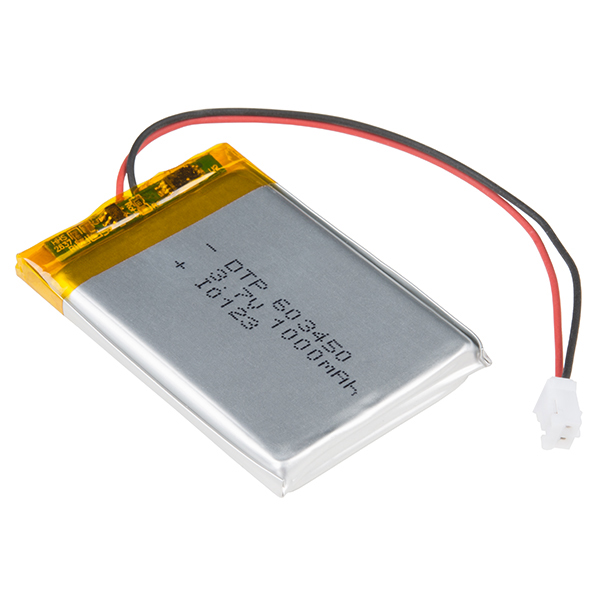
\includegraphics[width=100pt]{images/batt_lipo}
		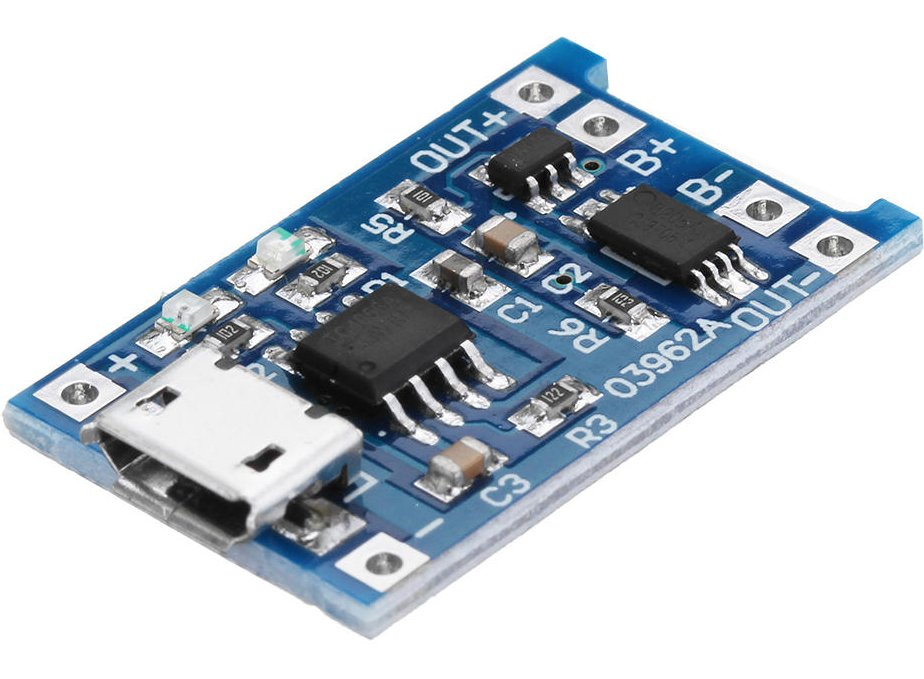
\includegraphics[width=100pt]{images/batt_tp4056}
		\caption{Contoh battery (kiri ke kanan): PP3 (9v), AAA(1.5V),LiPO 1000mAh, dan USB charging module}
	\end{figure}

	Untuk kompatibilitas chip, maka perlu dipertimbangkan kriteria berikut berikut:
	\begin{itemize}
		\item STM32F-series ARM32 Cortex-M
		\item Paket Chip LQFP64
		\item I2S interface minimal 1
		\item SPI interface minimal 2
		\item USB-Device minimal 1
	\end{itemize}

	Maka berdasarkan kriteria di atas, berikut daftar chip yang kompatibel:
	\begin{itemize}
		\item STM32F072R8 dan STM32F072RB
		\item STM32F103RC hingga STM32F103RG
		\item STM32F303RB hingga STM32F303RE
		\item STM32F401RB hingga STM32F401RE
		\item STM32F411RC dan STM32F411RE 
		\item STM32F446RC dan STM32F446RE
	\end{itemize}
	
	\newpage
	\subsubsection{Pro-Cons}
	Berikut adalah beberapa poin keuntungan dan kerugian dari versi ini:\\
	
	\textbf{Pros}:
	\begin{itemize}
		\item Single PCB/Board tanpa perlu tambahan modul/board terpisah
		(kecuali USB charging module jika menggunakan rechargeable LiPO battery).
		
		\item Dengan kebutuhan minimum clearance 0.5mm dan paket komponen/pin terkecil adalah SMD QFP-64,
		PCB versi ini masih dapat diproduksi oleh PCB House lokal baik dengan masking maupun tidak.
		
		\item Pengadaan komponen relatif mudah didapat di lokal Surabaya.
		
		\item Dirancang untuk lebih kepada penggunaan \textit{end-user} dan lebih \textit{user convenience}.
	\end{itemize}
	
	\textbf{Cons}:
	\begin{itemize}
		\item Pertimbangan size dan space, hanya pas untuk satu modul MAX98357A, sehingga hanya mampu mono audio.
		\item Memiliki banyak vias di PCB sehingga membutuhkan waktu lebih lama untuk assembly jika dikerjakan manual. 
	\end{itemize}
	
	\subsubsection{3D Mock-Up}
	\begin{figure}[!ht]
		\centering
		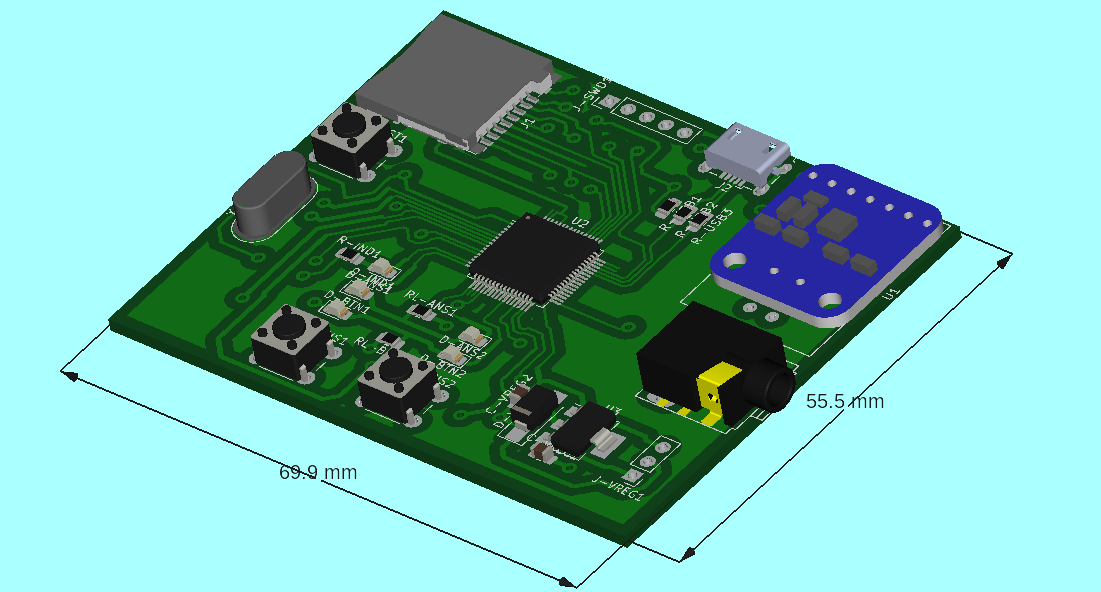
\includegraphics[width=400pt]{images/test2}
		\caption{Mock-Up 3D}
	\end{figure}

%%%%%%%%%%%%%%%%%%%%%%%%%%%%%%%%%%%%%%%%%%%%%%%%%%%%%%%%%%%%%%%%%

	\newpage
	\subsection{High Fabrication Version}
	
	\subsubsection{Features}
	\begin{figure}[!ht]
		\centering
		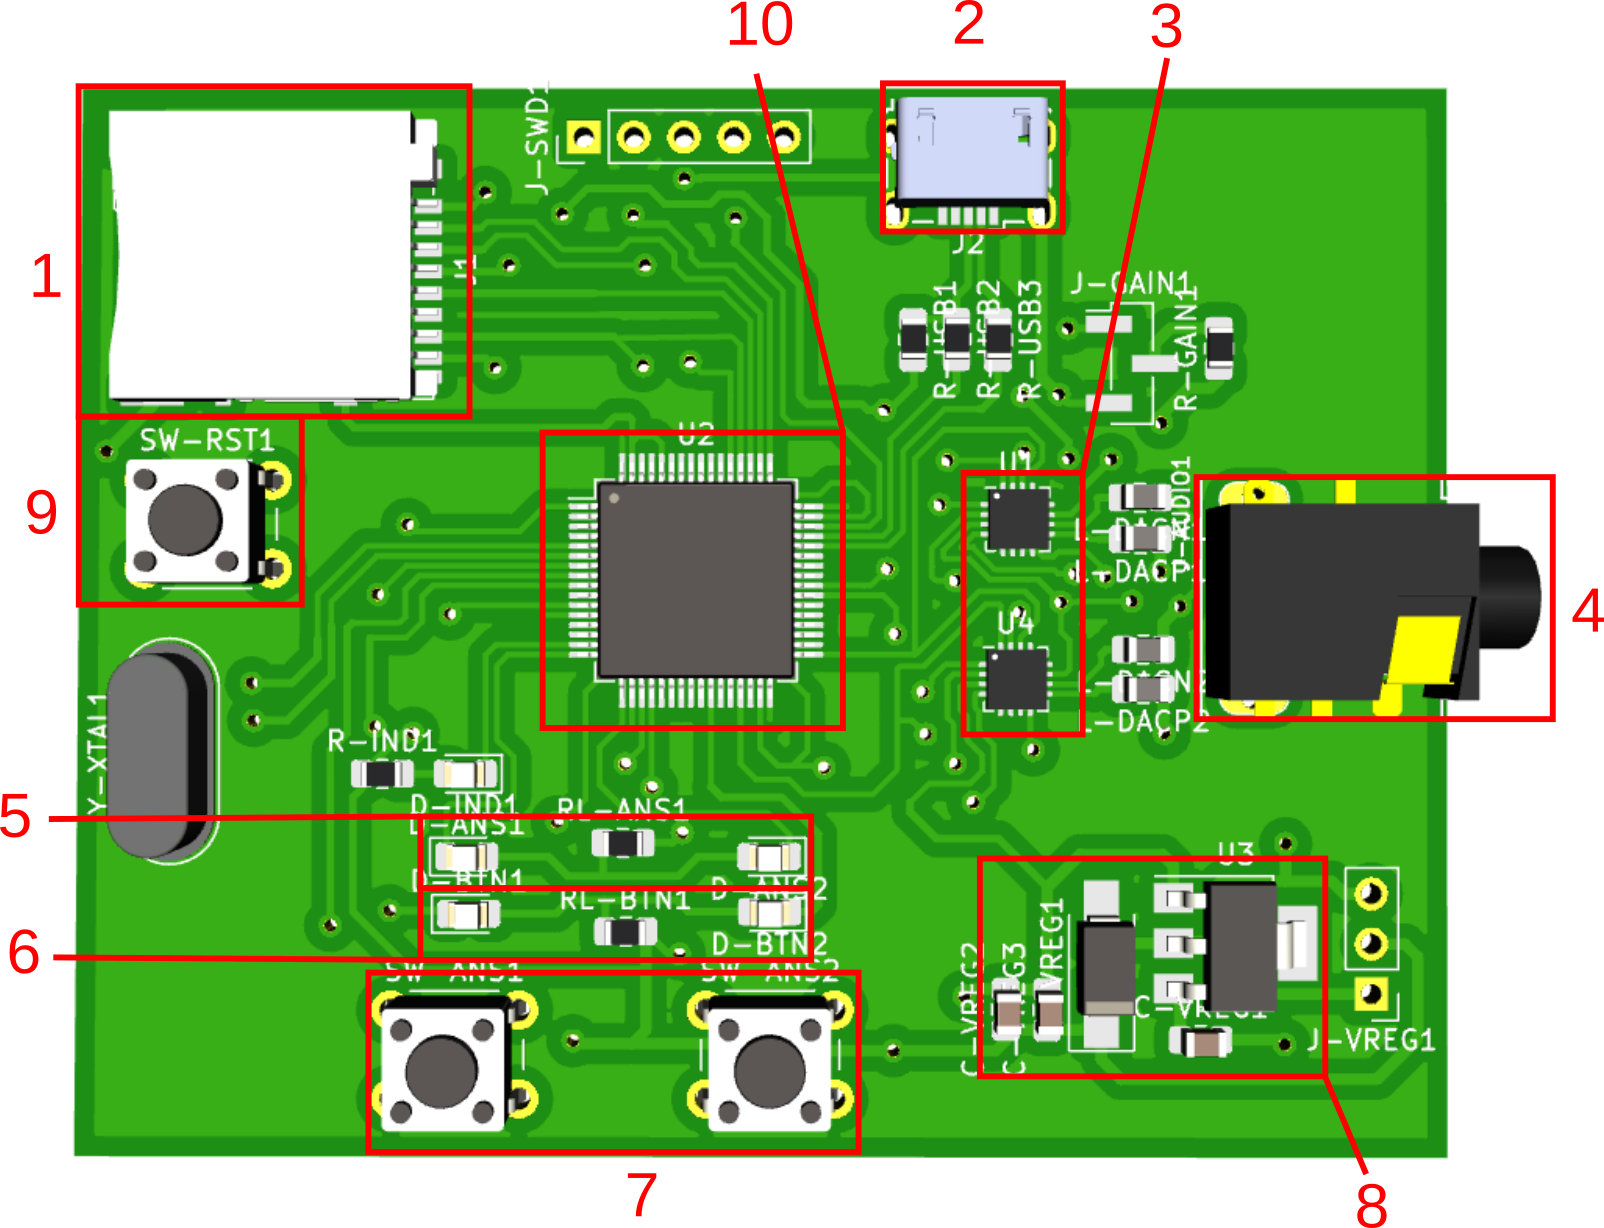
\includegraphics[width=500pt]{images/vhifab.png}
		\caption{Fitur dalam desain}
	\end{figure}

	Berikut adalah daftar fitur yang telah tersedia dalam desain:
	\begin{enumerate}
		\item \textbf{MicroSD slot.}\\
		Digunakan untuk menyimpan rekaman setiap sesi test dalam bentuk file teks.
		Format data dapat berupa CVS, XML, JSON, atau format data yang dibuat sendiri sesuai kebutuhan.
		
		\item \textbf{USB-Port.}\\
		USB Port untuk komunikasi dengan standar USB-CDC (Communication Device Class), yaitu emulasi komunikasi data serial.
		Kompatibel dengan driver ACM (Abstract Control Model) untuk Unix (Android/Linux) dan Usbser.sys untuk Windows.\\
		Beberapa varian main CPU chip juga menyediakan USB-OTG-FS Host untuk handle USB Flash-Disk (implementasinya sedang direncanakan).
				
		\newpage
		\item \textbf{Max98357A Chip.}\\
		Audio DAC (Digital to Analog Converter) MAX98357A adalah \textbf{Mono Class-D} amplifier untuk menghasilkan Audio output dengan input
		PCM (Pulse-Coded Modulation) standar I2S (Inter-IC Sound).\\
		\textbf{Spesifikasi}: 86-11800 Hz dan 98-42 dB pada default amplifikasi 9dB (Diukur menggunakan KEMAR-set dan Audio-Box BSWA).\\
		Dalam versi ini, menggunakan chip berpaket QFN-16 sehingga cukup space untuk 2 chip dan menyediakan output dual (bukan stereo). 
		
		\item \textbf{Jack Audio.}\\ 
		Jack Audio 3.5mm dengan konfigurasi pin TRS (Tip,Round,Sleeve) dan kompatibel untuk jack TRRS OMTP/Nokia.
		
		\item \textbf{LED True/False Indicator.}\\
		LED ukuran SMD 0805 sebagai indikator jawaban salah atau benar.
		
		\item \textbf{LED Answer Options Indicator.}\\
		LED ukuran SMD 0805 sebagai indikator jawaban pilihan jawaban untuk user.
		
		\item \textbf{User-Button Answer Options.}\\
		Tombol untuk input user terhadap jawaban.
		
		\item \textbf{Power/Voltage Regulator}\\
		Set voltage regulator berbasis IC AM1117 untuk regulasi tegangan input dari 5-12 volt ke VDD (3.3 volt) pada maksimal arus 1A.
		Battery monitor/charging circuit direncanakan masih menggunakan modul terpisah.
		
		\item \textbf{Reset Button.}\\
		Tombol input user untuk mengulang proses running/testing dari unit.
		
		\item \textbf{Main CPU STM32F-series.}\\
		Main microcontroller chip sebagai CPU. Menggunakan chip seri STM32F pada arsitektur ARM32 Cortex-M0/M3/.
		
	\end{enumerate}

	\subsubsection{Power-Compats}
	
	Untuk power, sama dengan versi sebelumnya, meliputi \textit{one-use} battery semisal battery PP3 (9v) atau AAA dalam 3-in-series,
	sedangkan untuk \textit{rechargable} battery dapat menggunakan 1000mAh dengan dilengkapi modul monitor/charging berbasis IC TP-4056.
	
	\begin{figure}[!ht]
		\centering
		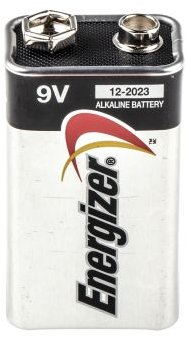
\includegraphics[width=50pt]{images/batt_pp3}
		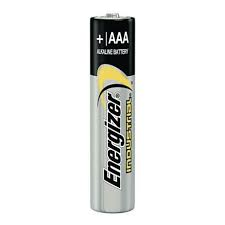
\includegraphics[width=100pt]{images/batt_aaa}
		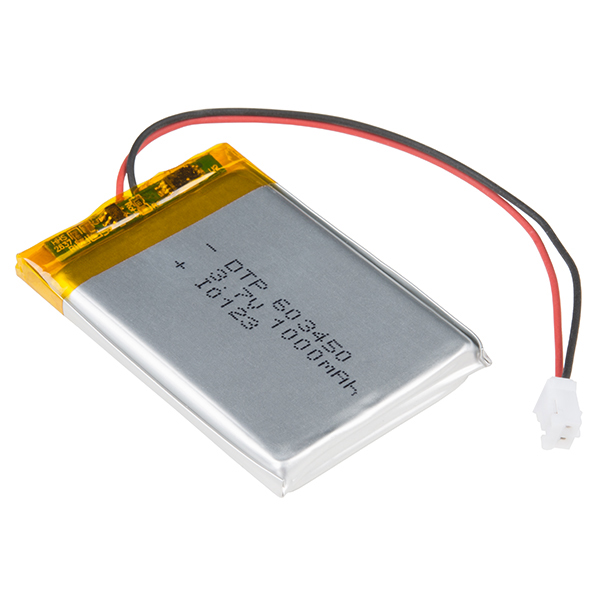
\includegraphics[width=100pt]{images/batt_lipo}
		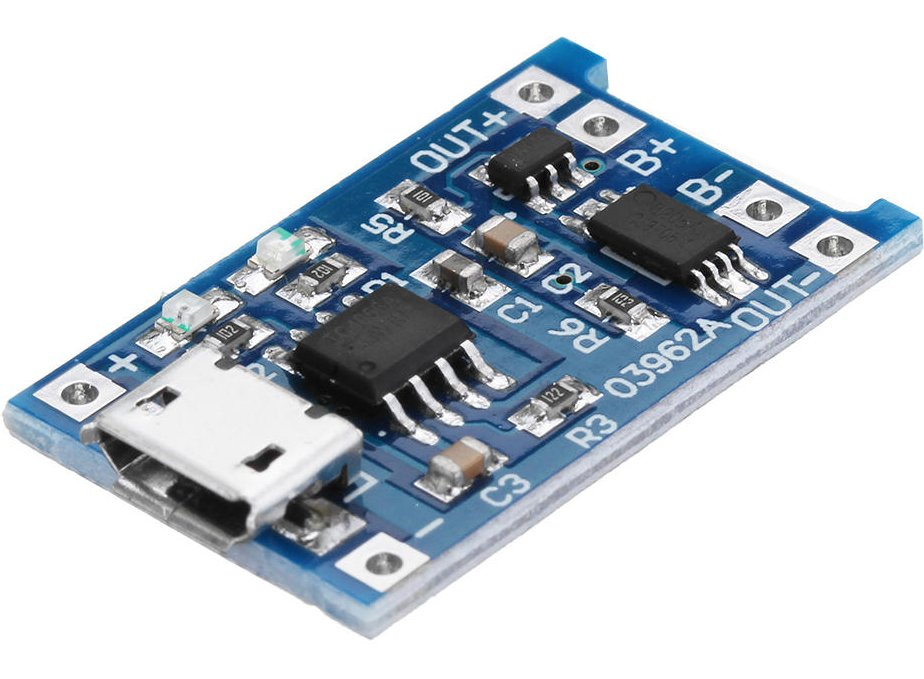
\includegraphics[width=100pt]{images/batt_tp4056}
		\caption{Contoh battery (kiri ke kanan): PP3 (9v), AAA(1.5V),LiPO 1000mAh, dan USB charging module}
	\end{figure}

	Untuk kompatibilitas chip juga sama dengan versi sebelumnya, meliputi:
	\begin{itemize}
		\item STM32F072R8 dan STM32F072RB
		\item STM32F103RC hingga STM32F103RG
		\item STM32F303RB hingga STM32F303RE
		\item STM32F401RB hingga STM32F401RE
		\item STM32F411RC dan STM32F411RE 
		\item STM32F446RC dan STM32F446RE
	\end{itemize}
	
	\newpage	
	\subsubsection{Pro-Cons}
	Berikut adalah beberapa poin keuntungan dan kerugian dari versi ini:\\
	
	\textbf{Pros}:
	\begin{itemize}
		\item Single PCB/Board tanpa perlu tambahan modul/board terpisah
		(kecuali USB charging module jika menggunakan rechargeable LiPO battery).
		
		\item Dengan kebutuhan minimum clearance 0.5mm, PCB masih dapat diproduksi oleh PCB House lokal
		
		\item Tersedia untuk 2 chip MAX98357A sehingga mampu output dual (bukan stereo).
		
		\item Dirancang untuk lebih kepada penggunaan \textit{end-user} dan lebih \textit{user convenience}.
	\end{itemize}
	
	\textbf{Cons}:
	\begin{itemize}
		\item Membutuhkan PCB House atau PCB Manufaktur/Fabrication dengan \textit{requirement} lebih tinggi,
		dikarenakan diameter vias lebih kecil, jumlah vias jauh lebih banyak, dan wajib through-hole saat fabrikasi.
		PCB House/Fabrication dengan kapabilitas ini terbatas di lokal dan waktu pengerjaan lebih lama serta harga per batch order cenderung lebih mahal. 
		
		\item Chip MAX98357A berpaket QFN-16 non-module, sehingga untuk soldering memerlukan teknik solder hot-air dan mewajibkan PCB yang di-\textit{masking}.
	
		\item Ketersediaan chip MAX98357A dalam paket QFN-16 (bukan modul) sangat terbatas dan ada kemungkinan perlu impor sendiri.
	\end{itemize}

	\subsubsection{3D Mock-Up}
	\begin{figure}[!ht]
		\centering
		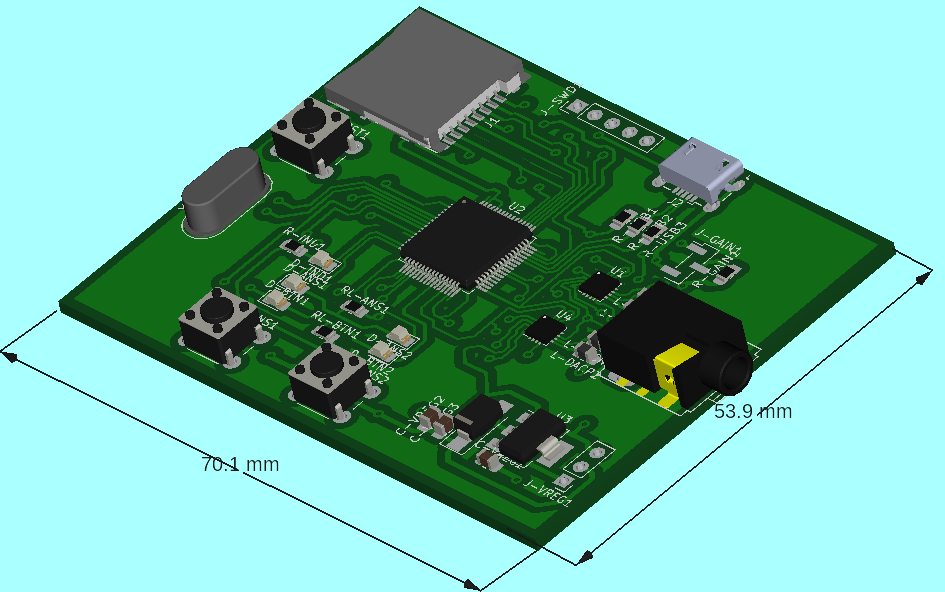
\includegraphics[width=400pt]{images/test3}
		\caption{Mock-Up 3D}
	\end{figure}
	
%%%%%%%%%%%%%%%%%%%%%%%%%%%%%%%%%%%%%%%%%%%%%%%%%%%%%%%%%%%%%%%%%	
	
	\newpage
	\section{Standard Requirements} 
	
	Berikut beberapa standard terkait Alat Kesehatan (Alkes) atau Medical-Instrument, dan Audiometri.
	Poin-poin utama yang langsung terkait dengan proses development masih dalam proses dipelajari.
	
	\subsection{Safety}
	
	\subsubsection{EN 60601-1:2006+AC:2010}
	Medical devices Directive (93/42/EEC):\\
	Medical electrical equipment - Part 1: General requirements for basic safety and essential performance.\\
	
	Source URLs:
	\begin{itemize}
		\item Webpage:\\
		\url{https://ce-marking.help/directive/medical-devices/standard/3527/en-60601-12006ac2010}
		
		\item Directive-PDF:\\
		\url{https://ce-marking.help/pdf/Directives/MDD\%20Directive\%2093_42.pdf}
	\end{itemize}

	\subsubsection{EN 60601-1-8:2007+AC:2010}
	Medical devices Directive (93/42/EEC):\\
	Medical electrical equipment - Part 1-8: General requirements for basic safety and essential performance - 
	Collateral Standard: General requirements, tests and guidance for alarm systems in medical electrical equipment
	and medical electrical systems.\\ 
	
	Source URLs:
	\begin{itemize}
		\item Webpage:\\
		\url{https://ce-marking.help/directive/medical-devices/standard/3538/en-60601-1-82007ac2010}
		
		\item Directive-PDF (idem).
	\end{itemize}

	\subsection{Audiometri}
	
	\subsubsection{EN 60645-1:2001}
	Medical devices Directive (93/42/EEC):\\
	Electroacoustics - Audiological equipment - Part 1: Pure-tone audiometers\\
	
	Source URLs:
	\begin{itemize}
		\item Webpage:\\
		\url{https://ce-marking.help/directive/medical-devices/standard/3601/en-60645-12001}
		
		\item Standard-PDF:\\
		\url{https://ce-marking.help/harmonised_standard/pdf/directive/medical-devices/st/3601/EN_60645_1_2001.pdf}
		
		\item Directive-PDF (idem).
	\end{itemize}

	\subsubsection{EN 60645-2:1997}
	Medical devices Directive (93/42/EEC):\\
	Audiometers - Part 2: Equipment for speech audiometry\\
	
	Source URLs:
	\begin{itemize}
		\item Webpage:\\
		\url{https://ce-marking.help/directive/medical-devices/standard/3602/en-60645-21997}
		
		\item Standard-PDF:\\
		\url{https://ce-marking.help/harmonised_standard/pdf/directive/medical-devices/st/3602/EN_60645_2_1997.pdf}
		
		\item Directive-PDF (idem).
	\end{itemize}

	\subsubsection{EN 60645-4:1995}
	Medical devices Directive (93/42/EEC):\\
	Audiometers - Part 4: Equipment for extended high-frequency audiometry\\
	
	Source URLs:
	\begin{itemize}
		\item Webpage:\\
		\url{https://ce-marking.help/directive/medical-devices/standard/3604/en-60645-41995}
		
		\item Standard-PDF:\\
		\url{https://ce-marking.help/harmonised_standard/pdf/directive/medical-devices/st/3604/EN_60645_4_1995.pdf}
		
		\item Directive-PDF (idem).
	\end{itemize}
	
	\subsection{Calibration}
	
	\subsubsection{EN 389-1}
	Acoustics - Reference zero for the calibration of audiometric equipment:\\
	Part 1: Reference equivalent threshold sound pressure levels for pure tones and supra-aural earphones.\\
	
	Source URLs:
	\begin{itemize}
		\item Webpage:\\
		\url{https://www.techstreet.com/standards/din-en-iso-389-1?product_id=2015882}
		
		\item Standard-PDF is paid item.
	\end{itemize}

	\subsubsection{EN 389-3}
	Acoustics - Reference zero for the calibration of audiometric equipment:\\
	Part 3: Reference equivalent threshold force levels for pure tones and bone vibrators.\\
	
	Source URLs:
	\begin{itemize}
		\item Webpage:\\
		\url{https://www.techstreet.com/standards/din-en-iso-389-3?product_id=1917960}
		
		\item Standard-PDF is paid item.
	\end{itemize}

	\subsubsection{EN 389-4}
	Acoustics - Reference zero for the calibration of audiometric equipment:\\
	Part 4: Reference levels for narrow-band masking noise.\\
	
	Source URLs:
	\begin{itemize}
		\item Webpage:\\
		\url{https://www.techstreet.com/standards/din-en-iso-389-4?product_id=1072540}
		
		\item Standard-PDF is paid item.
	\end{itemize}

	\subsubsection{EN 389-5}
	Acoustics - Reference zero for the calibration of audiometric equipment:\\
	Reference equivalent threshold sound pressure levels for pure tones in the frequency range 8 kHz to 16 kHz.\\
	
	Source URLs:
	\begin{itemize}
		\item Webpage:\\
		\url{https://www.techstreet.com/standards/din-en-iso-389-5?product_id=1376080}
		
		\item Standard-PDF is paid item.
	\end{itemize}

	\subsubsection{EN 389-7}
	Acoustics - Reference zero for the calibration of audiometric equipment:\\
	Reference threshold of hearing under free-field and diffuse-field listening conditions.\\
	
	Source URLs:
	\begin{itemize}
		\item Webpage:\\
		\url{https://www.techstreet.com/standards/din-en-iso-389-7?product_id=1940002}
		
		\item Standard-PDF is paid item.
	\end{itemize}

	\subsubsection{ANSI/ASA S3.6-2018 }
	The audiometers covered in this specification are devices designed for use in determining the hearing threshold
	of an individualin comparison with a chosen standard reference threshold level.\\
	This standard provides specifications and tolerances for pure-tone, speech,
	and masking levels and describes the minimum test capabilities of different types of audiometers.\\
	The standard also specifies standardized threshold for detecting pure tones.\\
	
	Source URLs:
	\begin{itemize}
		\item Webpage:\\
		\url{https://www.techstreet.com/standards/asa-s3-6-2018?product_id=2027721}\\
		
		\item Abstract:\\
		\url{https://www.ncbi.nlm.nih.gov/books/NBK207830/}
		
		\item Standard-PDF is paid item.
	\end{itemize}

\end{document}